\documentclass[11pt,aspectratio=43,usenames,dvipsnames]{beamer}
\usepackage[utf8]{inputenc}
\usepackage{amsmath, amsfonts, amssymb, amsthm}
\usepackage[T1]{fontenc}
% mint: code chuck and syntax highlighting
%% outputdir should change according to pdf build directory
\usepackage[outputdir=build,cache=false]{minted}
\usepackage{lmodern}
\usepackage{xcolor}
\usepackage{setspace}
\usepackage{booktabs}
\usepackage{multirow}
\usepackage{graphicx}
\usepackage{fontawesome}

\usepackage[mode=tex]{standalone}
\usepackage{tikz}
\usetikzlibrary{decorations}
\usetikzlibrary{decorations.pathreplacing, intersections}
\usepackage{pgfplots}
\usetikzlibrary{calc,positioning}
\usepgfplotslibrary{fillbetween}
\pgfplotsset{compat=newest, scale only axis, width = 10cm}

% ---------------------------------------------------------------------
% Coordinate extraction
% #1: node name
% #2: output macro name: x coordinate
% #3: output macro name: y coordinate
\newcommand{\Getxycoords}[3]{%
    \pgfplotsextra{%
        % using `\pgfplotspointgetcoordinates' stores the (axis)
        % coordinates in `data point' which then can be called by
        % `\pgfkeysvalueof' or `\pgfkeysgetvalue'
        \pgfplotspointgetcoordinates{(#1)}%
        % `\global' (a TeX macro and not a TikZ/PGFPlots one) allows to
        % store the values globally
         \global\pgfkeysgetvalue{/data point/x}{#2}%
         \global\pgfkeysgetvalue{/data point/y}{#3}%
     }%
}
% ---------------------------------------------------------------------

\usepackage{ulem}
\usepackage{hyperref}
\usepackage{booktabs}
\usepackage{babel}
\usepackage{makecell}
\usepackage[para,online,flushleft]{threeparttable}
\usepackage{pdfpages}
\usepackage{tcolorbox}
\usepackage{bm}
\usepackage{appendixnumberbeamer}
\usepackage{natbib}
\usepackage{caption}
\captionsetup[figure]{labelformat=empty}% redefines the caption setup of the figures environment in the beamer class.
\usetheme[compress]{Boadilla}
\usecolortheme{default}
\useoutertheme{miniframes}
\usefonttheme[onlymath]{serif}

\newcommand{\jump}[2]{\hyperlink{#1}{\beamerbutton{#2}}}
\newcommand{\extjump}[2]{\href{#1}{\beamerbutton{#2}}}
\newcommand{\orange}[1]{\textcolor{orange}{#1}}
\newcommand{\red}[1]{\textcolor{red}{#1}}
\newcommand{\blue}[1]{\textcolor{blue}{#1}}
\newcommand{\green}[1]{\textcolor{OliveGreen}{#1}}

\renewcommand{\square}{\scalebox{0.7}{$\blacksquare$ \hspace{0.5em}}}
\setbeamertemplate{itemize item}{\raisebox{0.1em}{\scalebox{0.7}{$\blacksquare$}}}
\setbeamertemplate{itemize subitem}[circle]
\setbeamertemplate{itemize subsubitem}{--}
\setbeamercolor{itemize item}{fg=black}
\setbeamercolor{itemize subitem}{fg=black}
\setbeamercolor{itemize subsubitem}{fg=black}
\setbeamercolor{item projected}{bg=darkgray,fg=white}
\definecolor{blue}{rgb}{0.2, 0.2, 0.7}
\setbeamercolor{alerted text}{fg=blue}
\setbeamertemplate{enumerate items}[circle]


\setbeamertemplate{headline}{}

%==========================================
\let\olditemize=\itemize
\let\endolditemize=\enditemize
\renewenvironment{itemize}{\olditemize \itemsep1em}{\endolditemize}
\let\oldenumerate=\enumerate
\let\endoldenumerate=\endenumerate
\renewenvironment{enumerate}{\oldenumerate \itemsep1em}{ \endoldenumerate}

\DeclareMathOperator*{\argmax}{\arg\!\max}
\DeclareMathOperator*{\E}{\mathbb{E}}
\DeclareMathOperator*{\var}{\rm Var}
\DeclareMathOperator*{\cov}{\rm Cov}

\theoremstyle{definition}
\newtheorem{assume}{Assumption}
\newtheorem{lem}{Lemma}
\newtheorem{proposition}{Proposition}
\newtheorem{thm}{Theorem}
\newtheorem{corol}{Corollary}

\AtBeginSection[]{
  \begin{frame}[noframenumbering]
  \vfill
  \centering
  \begin{beamercolorbox}[sep=8pt,center,shadow=true,rounded=true]{title}
    \usebeamerfont{title}\insertsection\par%
  \end{beamercolorbox}
  \vfill
  \end{frame}
}

\begin{document}
    \title[Unit 15]{Unit 15 \\ Inflation, Unemployment and Monetary Policy}
    \author[Hui-Jun Chen]{Hui-Jun Chen}
    \institute[OSU]{The Ohio State University}
    \date{\today}
    \setbeamertemplate{navigation symbols}{}
    \setstretch{1.2}

%-------------------------------------------------------
{
%	\usebackgroundtemplate{\includegraphics[width=1\paperwidth]{../EveningSky_cropped_edit43_bright.jpg}}
    \begin{frame}
% \vspace{3em}
        \centering
%		{\footnotesize 	ECON 4002 Intermediate Macroeconomic Theory}
        \maketitle
% \vspace{-1.5em}
% \centering
% \includegraphics[width=0.55\linewidth]{Pictures/houses.jpeg}


    \end{frame}
}

% -------------------------------------------
\setbeamertemplate{headline}
{
\setbeamercolor{section in head/foot}{fg=black, bg=white}
\vskip1em \tiny \insertsectionnavigationhorizontal{1\paperwidth}{\hspace{0.50\paperwidth}}{}
}
%------------------------------------------

\section[Intro]{Introduction}
\label{sec:Introduction}

\begin{frame}{Introduction \extjump{https://www.core-econ.org/the-economy/book/text/15.html}{Textbook} \extjump{https://www.youtube.com/watch?v=EpMLAQbSYAw}{Age of Easy Money}}
\label{slide:Introduction}

\begin{itemize}
    \item \alert{Stable} economy is desirable, and the stabilizing \alert{price level} is the key
    \item \alert{Inflation} as the result of price level rises
    \item \alert{Phillips curve}: the trade-off between inflation and unemployment
    \item Central bank use \alert{monetary policy} in response to inflation
    \item Yet, there's some \alert{consequences} regarding Quantitative Easing:
    \begin{itemize}
        \item 2008 Great Recession $ \rightarrow  $ QE policy $ \rightarrow $ Money goes to financial mkt
        \item Moral Hazard: profit goes to my pocket, loss bailed out by Fed
        \item $ \Rightarrow  $ Too much money facilitates speculation: fragile financial system
        \item $ \Rightarrow  $ crypto hype \& crash (FTX); Silicon Valley Bank bank run
    \end{itemize}
\end{itemize}
\end{frame}

\section[\faMoney]{Inflation}
\label{sec:Inflation}

\begin{frame}{Key Concepts}
\label{slide:Key_Concepts}
    \begin{itemize}
        \item \textbf{Inflation}:  an increase in the general price level
        \item \textbf{Zero inflation}:  A constant price level from year to year
        \item \textbf{Deflation}:  A decrease in the general price level
        \item \textbf{Disinflation}:  A decrease in the rate of inflation
    \end{itemize}

    %
    \begin{equation*}
        \tag{The Fisher Equation}
        r = i - \pi
    ,\end{equation*}
    %
    where $ r $ is real interest rate, $ i $ is nominal interest rate, and $ \pi $ is inflation rate
\end{frame}

\begin{frame}{What's wrong with inflation?}
\label{slide:What_s_wrong_with_inflation_}
    \begin{itemize}
        \item Workers paid with fixed nominal income, $ \pi \uparrow  $ $ \Rightarrow  $ real income $ \downarrow  $.
        \item Inflation \alert{reduces the real} value of debt: borrowers \faSmileO \hspace{2pt} yet creditors \faFrownO .
        \item High rate of inflation makes the economy work less well:
        \begin{itemize}
            \item High inflation is often volatile → uncertainty
            \item Harder for producers: changes in \textbf{relative prices} or inflation?
            \item \textbf{menu costs} as firms have to update their prices more frequently
        \end{itemize}

    \end{itemize}

\end{frame}

\begin{frame}{What's wrong with deflation?}
\label{slide:What_s_wrong_with_deflation_}
    \begin{itemize}
        \item Deflation could cause worse consequences than high inflation.
        \item When price $ \downarrow  $, HH postpone consumption
        \begin{itemize}
            \item $ \because $ \alert{expect} goods to be cheaper in the future
            \item \alert{Increase} real debt burden, cut consumption for target wealth
        \end{itemize}
        \item $ \Rightarrow  $ negative shock to aggregate demand
    \end{itemize}
\end{frame}

\begin{frame}{Causes of inflation}
\label{slide:Causes_of_inflation}
    \begin{figure}
        \centering
        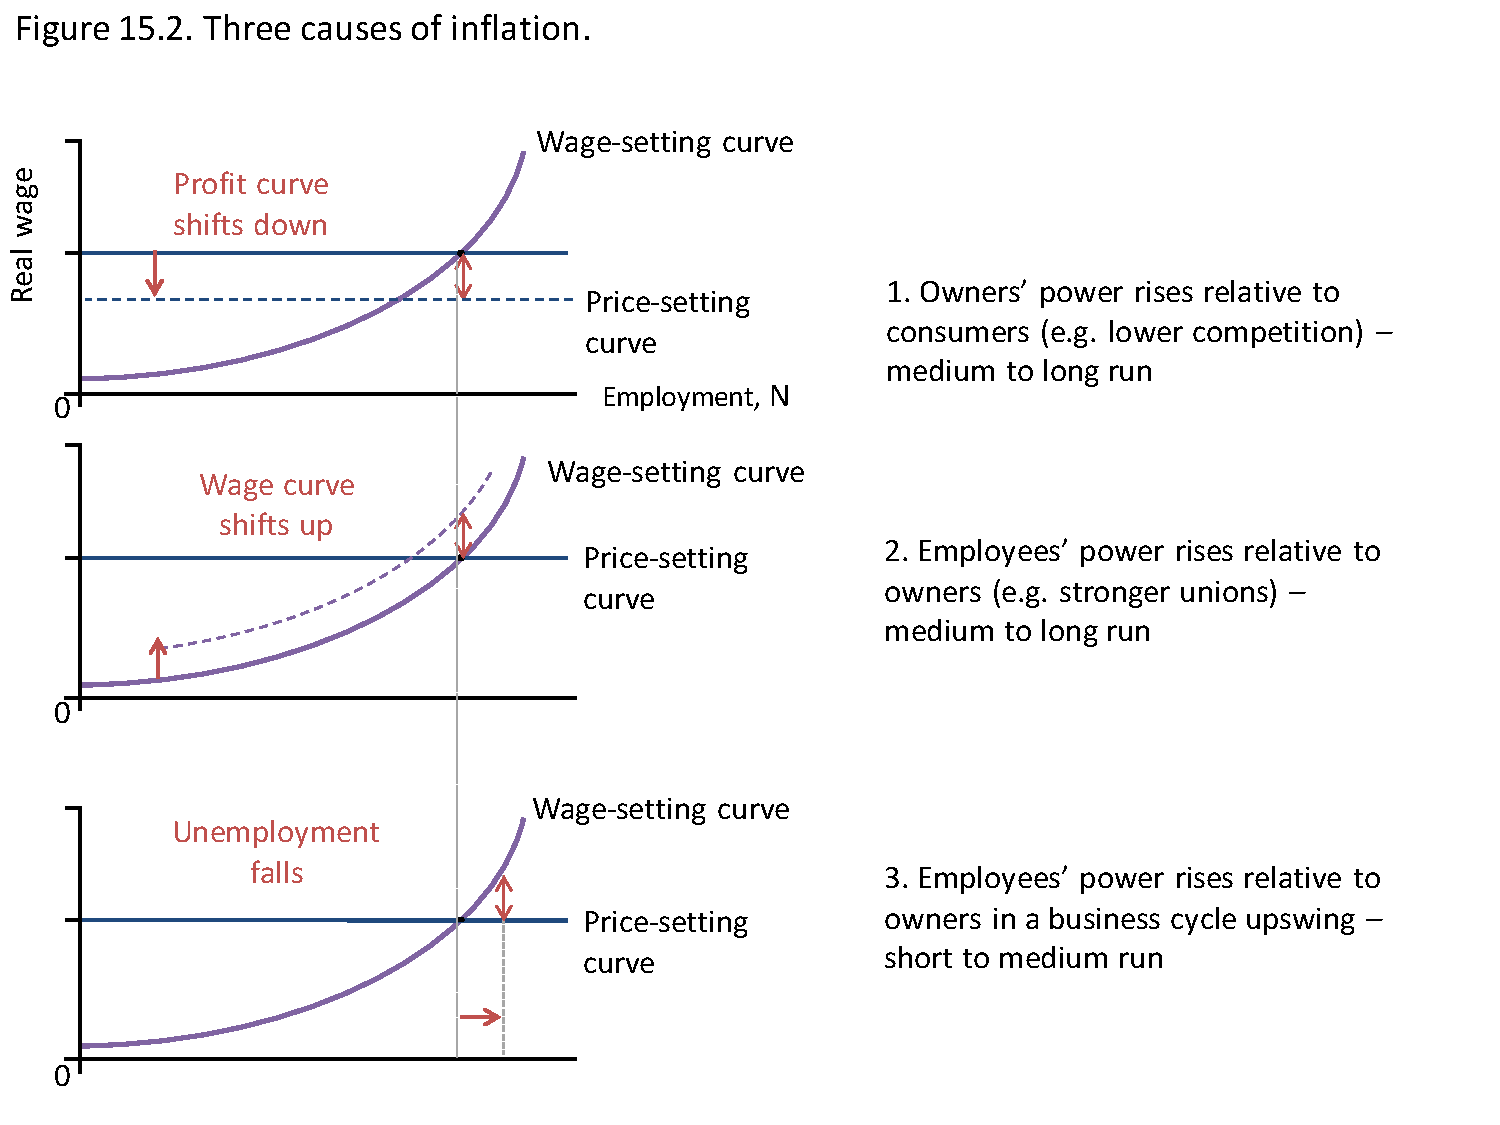
\includegraphics[width=.9\textwidth]{./figures/2.pdf}
    \end{figure}
\end{frame}

\section[\faObjectGroup]{Phillips Curve}
\label{sec:Phillips_Curve}

\begin{frame}{Inflation and unemployment}
\label{slide:Inflation_and_unemployment}

\begin{center}
    Unemployment $ \uparrow  $ $ \approx $ inflation $ \downarrow  $
\end{center}

\begin{itemize}
    \item increases workers' bargaining position → higher wages → higher cost of production → higher prices
\end{itemize}



\end{frame}

\begin{frame}{Inflation and Aggregate Demand}
\label{slide:Inflation_and_Aggregate_Demand}
    \begin{center}
         upswing in business cycle is often associated with rising inflation.
    \end{center}
    \begin{itemize}
        \item higher aggregate demand → higher employment → higher wages → higher cost of production → higher prices
        \item the economy experiences (nominal) price and wage inflation, but the \alert{real wage ($W/P$)} has not increased
        \item constant real wage means that employment stays high
        \item \ldots and the wage-price spiral continues

    \end{itemize}

\end{frame}

\begin{frame}{Stable price level}
\label{slide:Stable_price_level}
    \begin{center}
        Prices are stable ($\pi = 0$) when the labor market is in equilibrium.
    \end{center}
    \begin{columns}
        \begin{column}{0.3\textwidth}
            \begin{itemize}
                \item <only@1> Recall the labor productivity \& share of pie between worker and firm
                \item <only@1> Point $ A $ is labor market equilibrium
                \item <only@2> Point $ B $ is unemployment too low $ \Rightarrow  $ employment rent too low
                \item <only@2> Point $ C $ is unemployment too high $ \Rightarrow  $ firms hold too high bargaining power
                \item <only@3> Pt $ B $: workers' claims to real wages $ + $ firms' claims to real profits $ > $ total productivity → upward pressure on wages and prices
            \end{itemize}
        \end{column}
        \begin{column}{0.7\textwidth}
            \begin{figure}
                \centering
                \only<1>{
                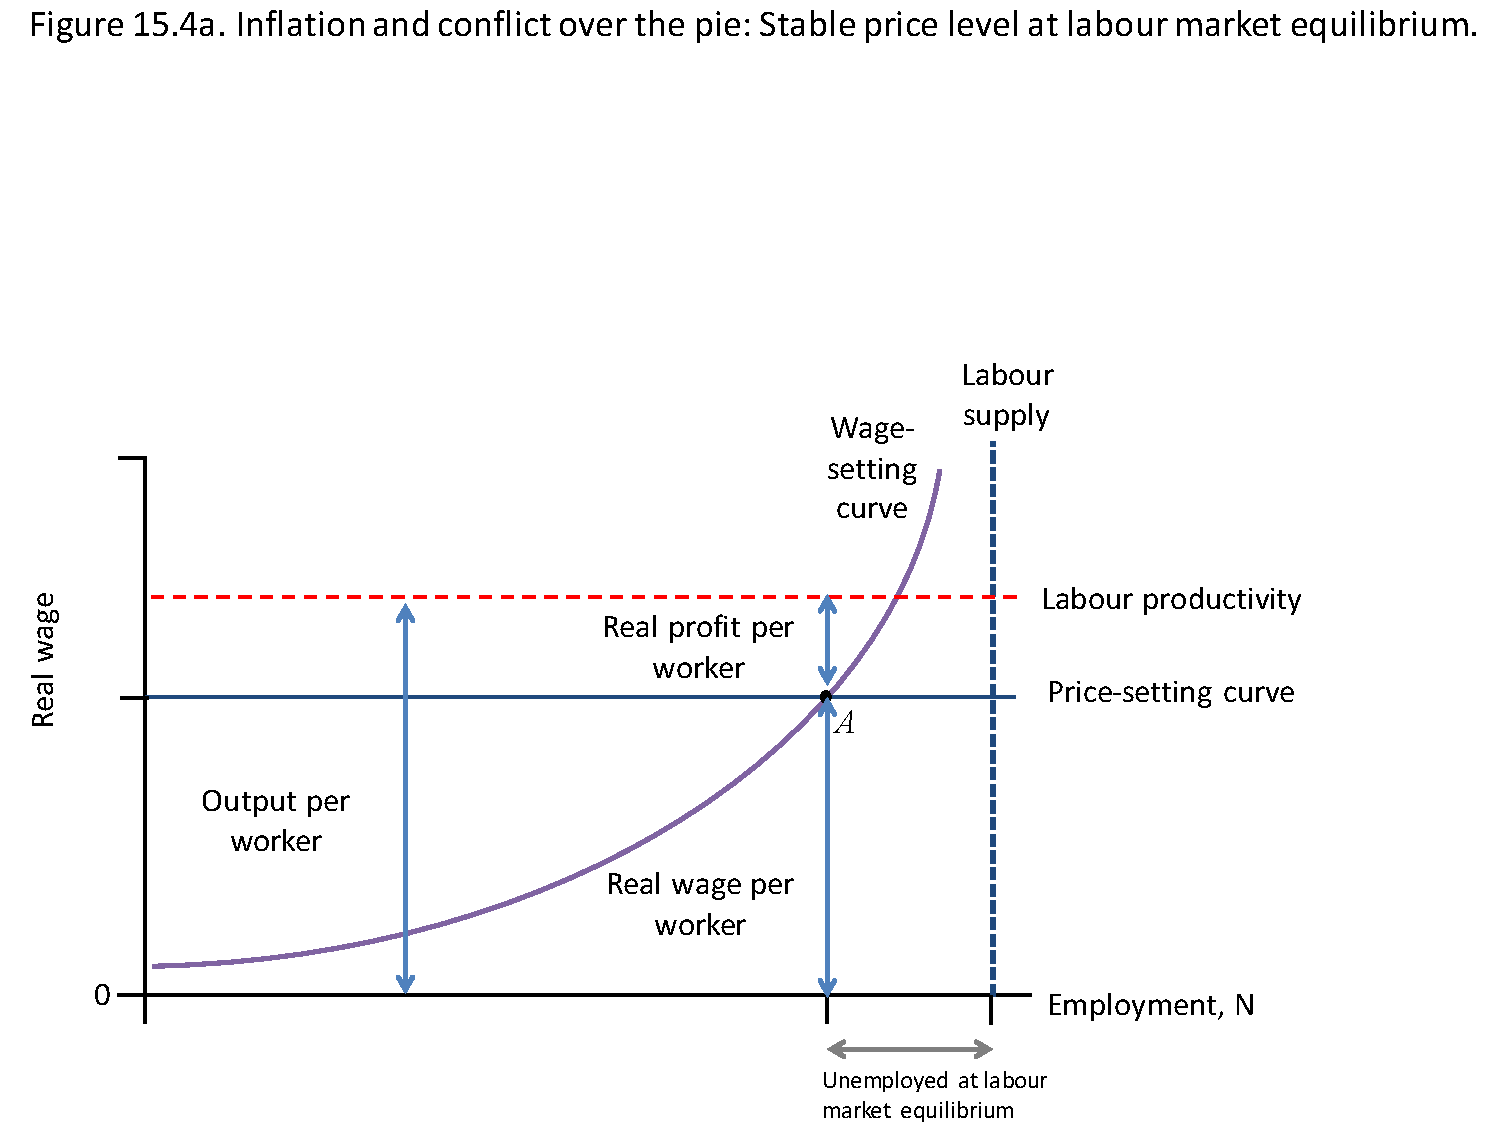
\includegraphics[width=\textwidth]{./figures/4.pdf}
                }
                \only<2-3>{
                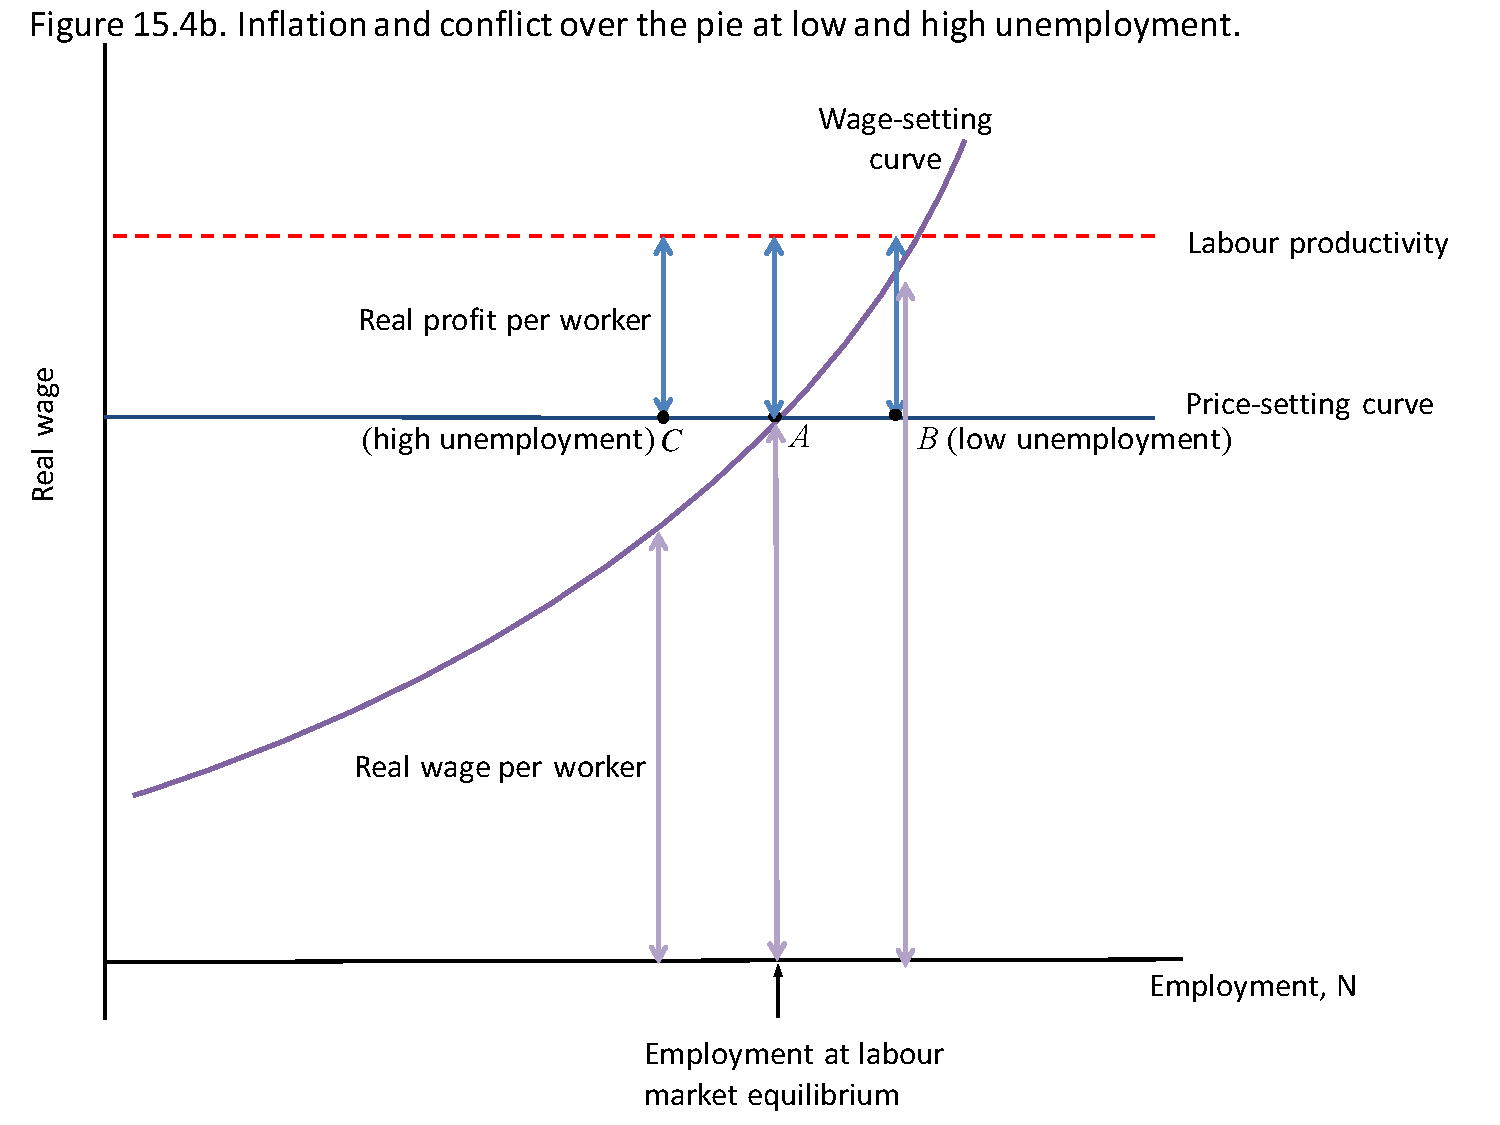
\includegraphics[width=\textwidth]{./figures/5.pdf}
                }
            \end{figure}

        \end{column}
    \end{columns}

\end{frame}

\begin{frame}{The bargaining gap}
\label{slide:The_bargaining_gap}
    \begin{itemize}
        \item \textbf{Bargaining gap}: The difference between the real wage required to incentivize effort, and the real wage that gives firms enough profits to stay in business.
        \item Unemployment is below equilibrium: a positive bargaining gap and inflation.
        \item Unemployment is above equilibrium: a negative bargaining gap and deflation.
        \item Labour market equilibrium: the bargaining gap is zero and the price level is constant.
    \end{itemize}
\end{frame}

\begin{frame}{Phillips Curve}
\label{slide:Phillips_Curve}
    \begin{figure}
        \centering
        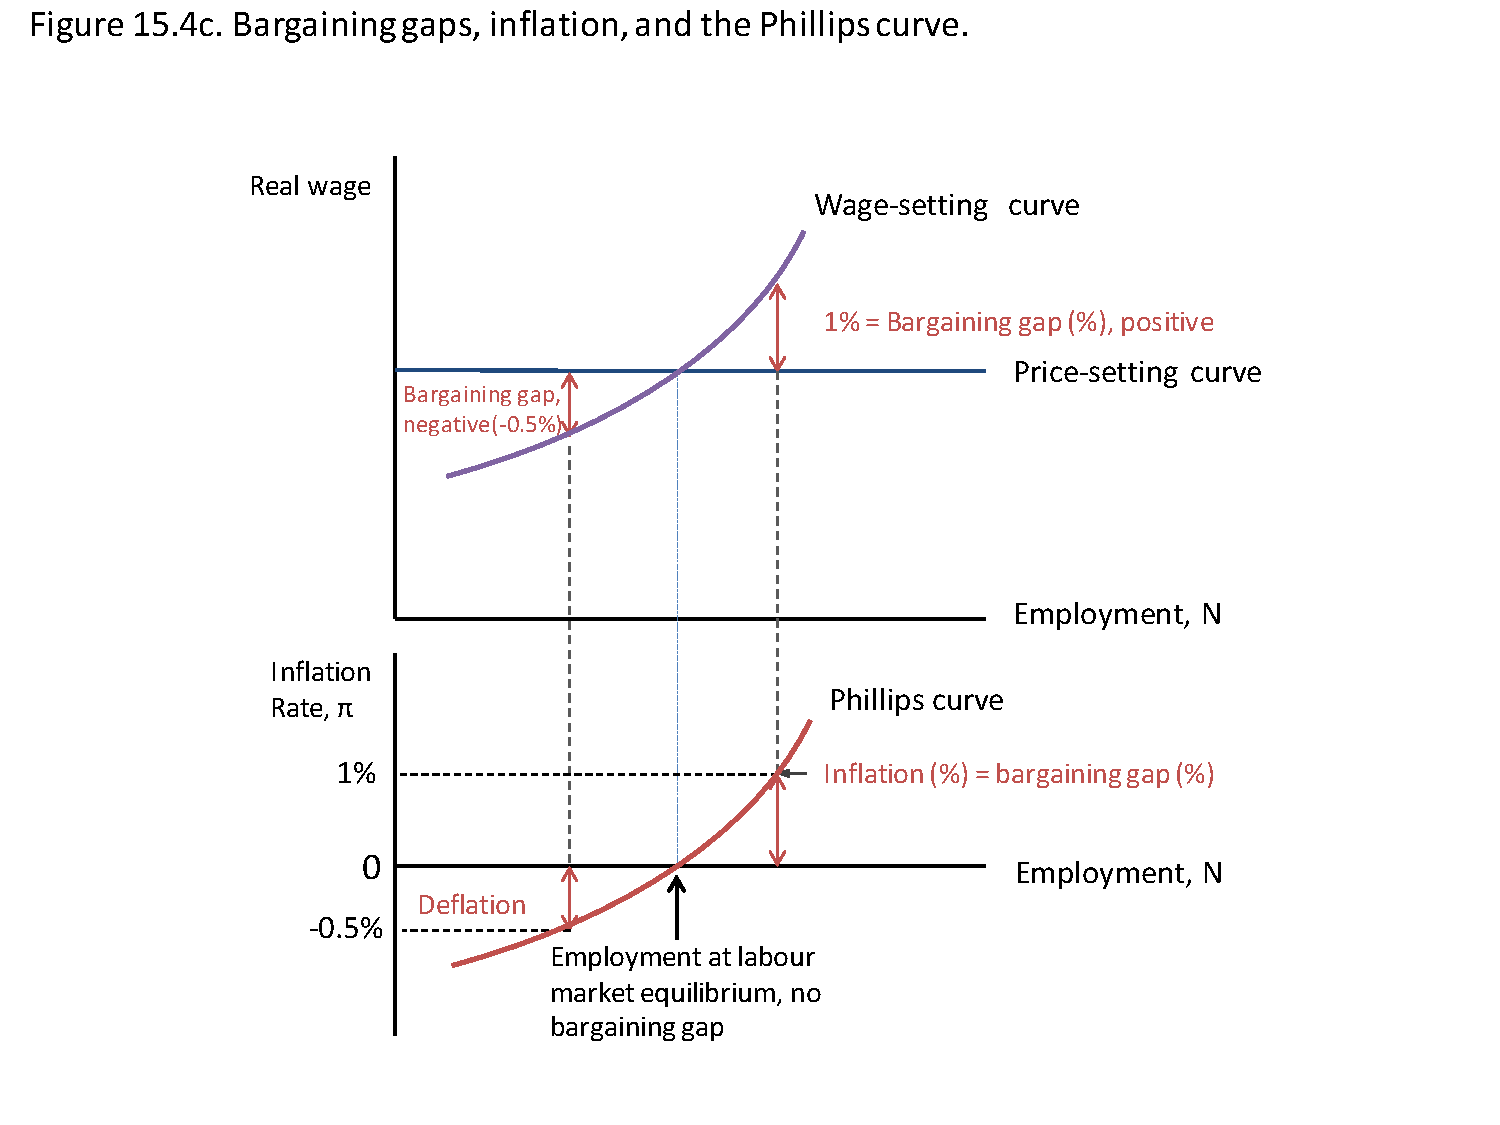
\includegraphics[width=.9\textwidth]{./figures/6.pdf}
    \end{figure}

\end{frame}

\begin{frame}{Phillips Curve and the Business Cycle}
\label{slide:Phillips_Curve_and_the_Business_Cycle}
    \begin{center}
        \only<1>{A positive bargaining gap in boom → inflation}
        \only<2>{A negative bargaining gap in recession → deflation}
    \end{center}
    \begin{figure}
        \centering
        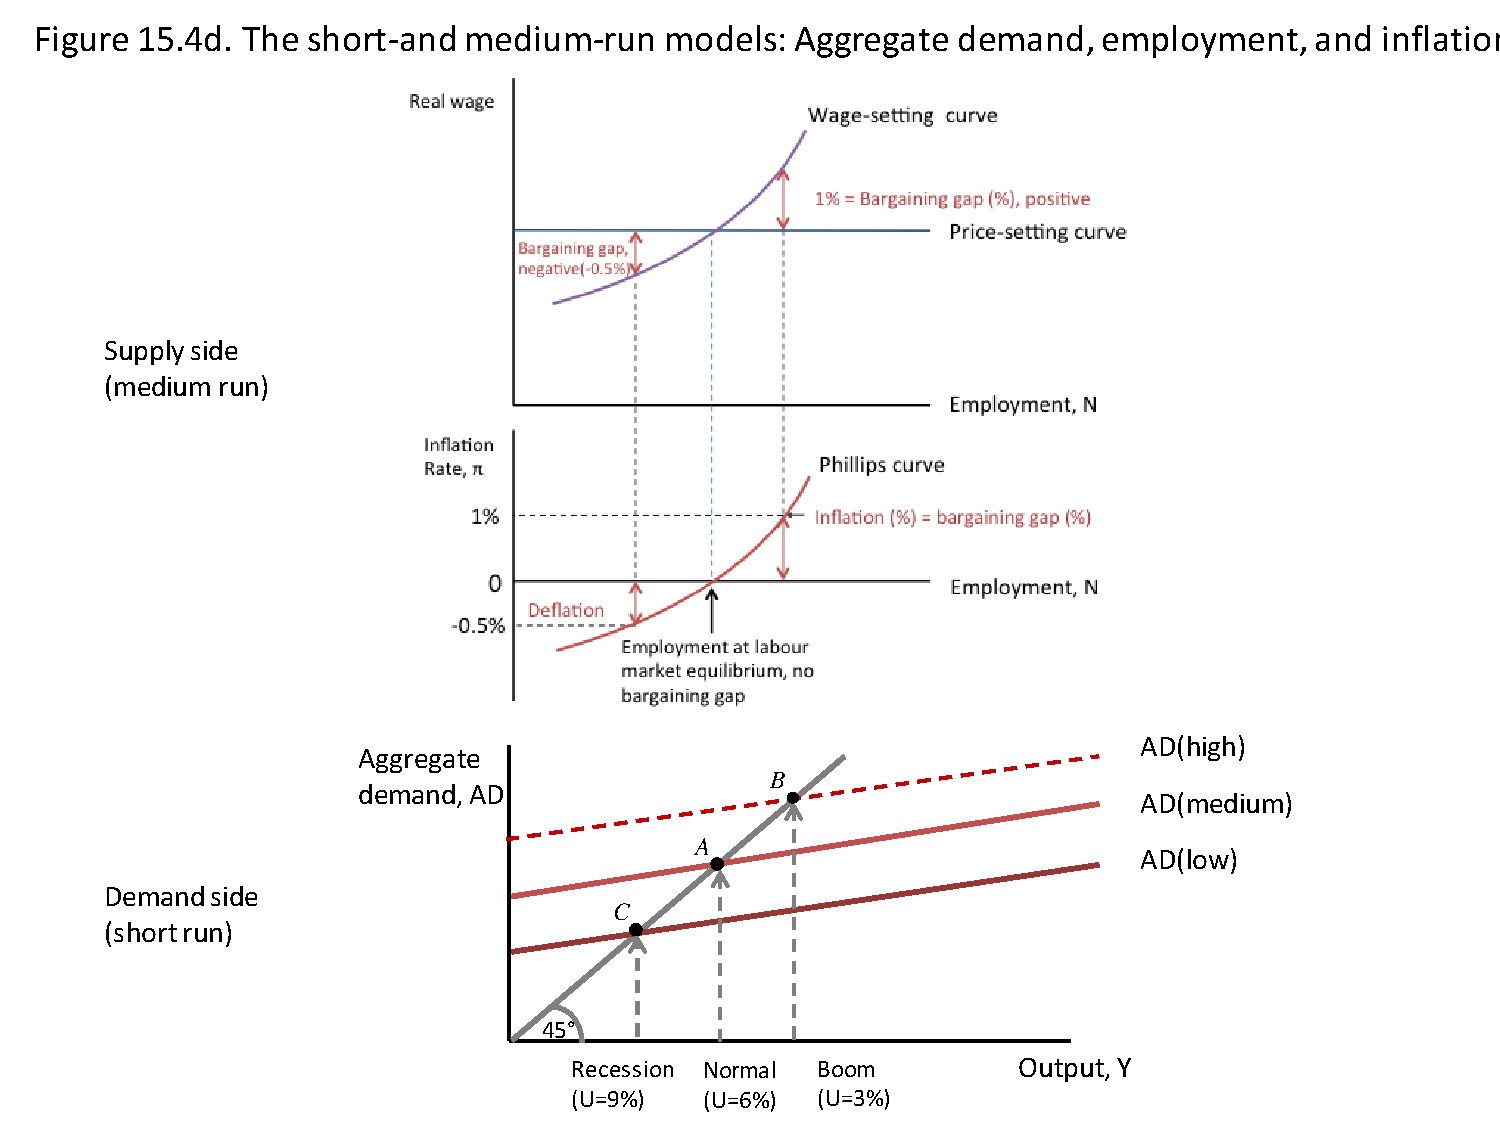
\includegraphics[width=.8\textwidth]{./figures/7.pdf}
    \end{figure}
\end{frame}

\begin{frame}{Central Bank's Decision}
\label{slide:Central_Bank_s_Decision}
    \begin{columns}
        \begin{column}{0.3\textwidth}
            \begin{itemize}
                \item<only@1> Phillips Curve determines the \alert{feasible trade-offs} between inflation and unemployment. (\textbf{MRT})
                \item<only@2> Indifference curves show \alert{policymaker’s preferred tradeoffs} between inflation and unemployment. (\textbf{MRS})
                \item<only@2> Target at $ 0\% $ unemployment $ \checkmark $
                \item<only@2> Target at $ 2\% $ inflation rate???
            \end{itemize}
        \end{column}
        \begin{column}{0.7\textwidth}
            \begin{figure}
                \centering
                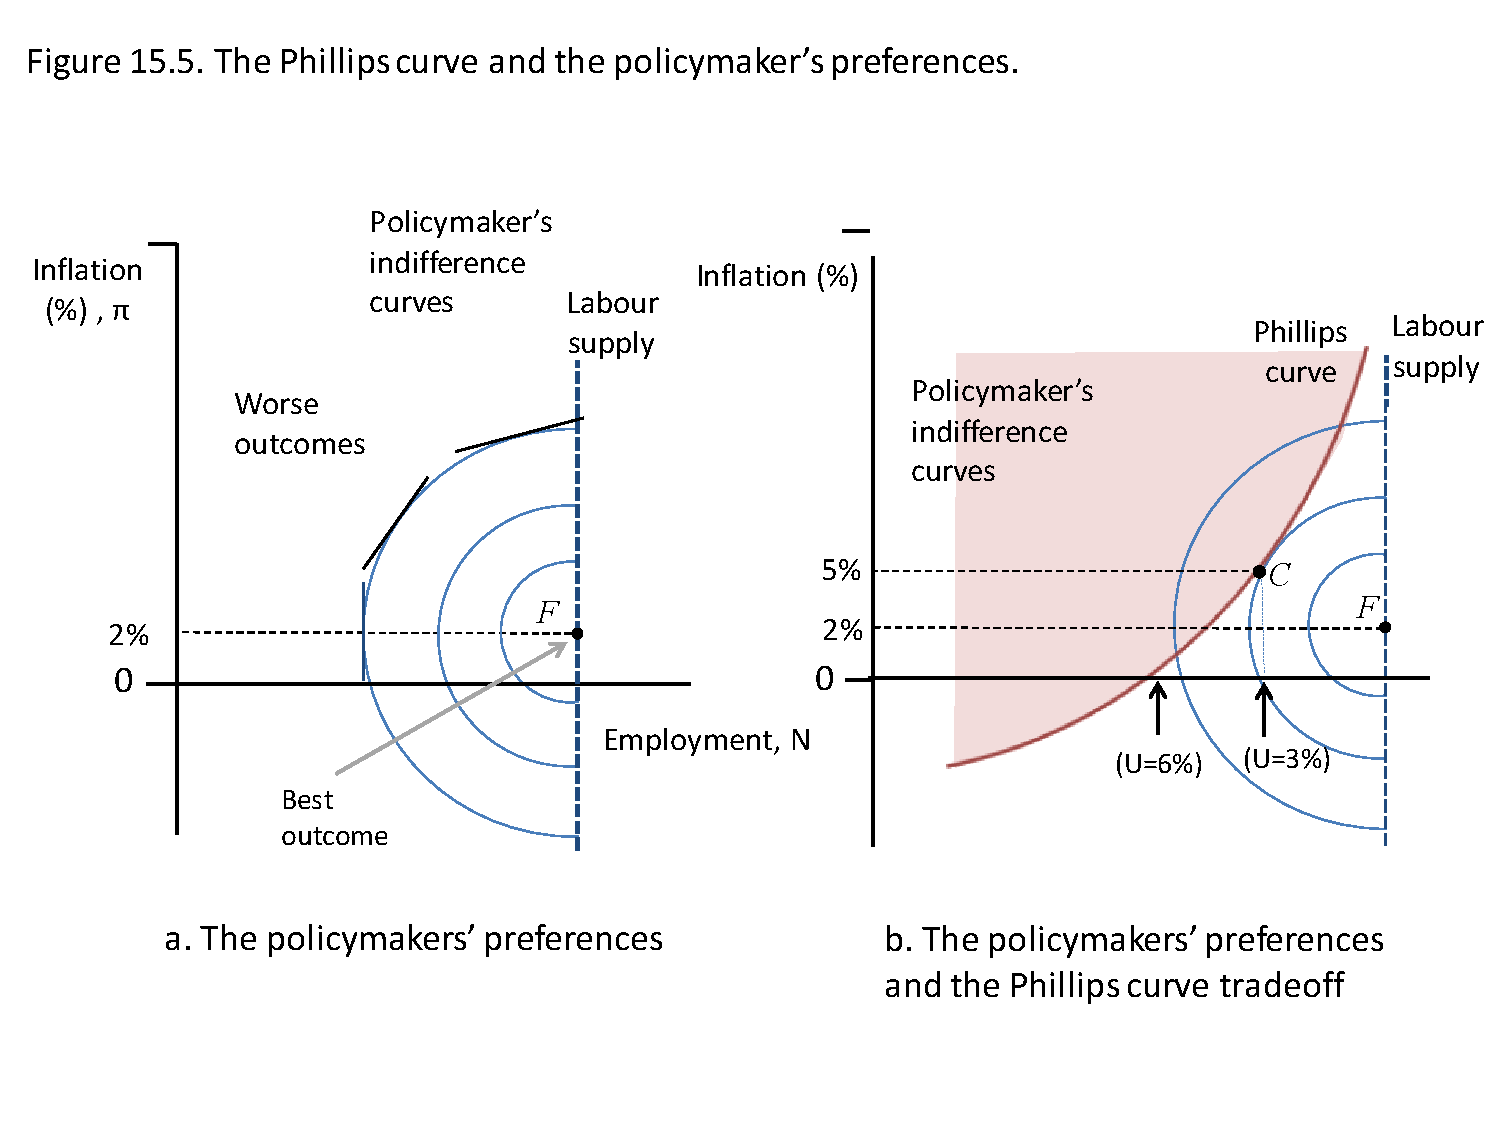
\includegraphics[width=\textwidth]{./figures/8.pdf}
                \only<2>{\caption{\extjump{https://youtu.be/UN-O6oNes0I}{What’s So Special About 2\% Inflation?}}}
            \end{figure}
        \end{column}
    \end{columns}
\end{frame}

\begin{frame}{Phillips Curve Over Time}
\label{slide:Phillips_Curve_Over_Time}
            \begin{itemize}
                \item Phillips Curve shifts over time
                \item Keeping unemployment ``too low'' leads to higher prices \& rising inflation
            \end{itemize}
            \begin{figure}
                \centering
                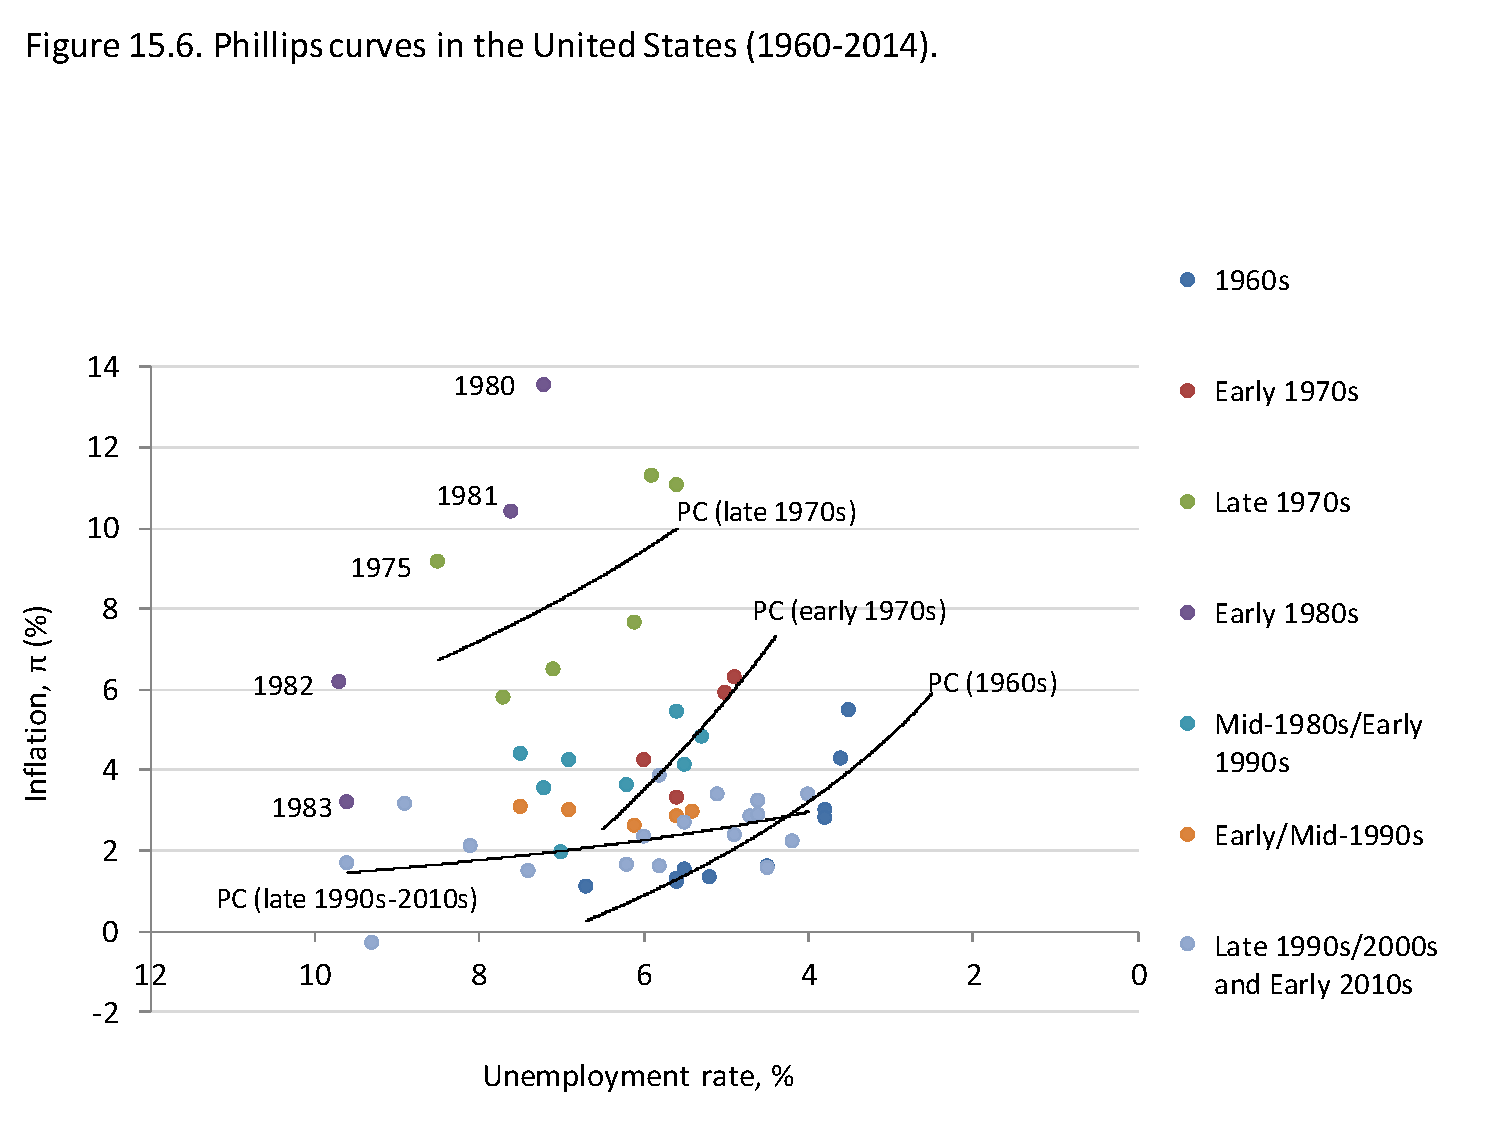
\includegraphics[trim={0cm 0cm 0cm 4.5cm}, clip, width=.8\textwidth]{./figures/9.pdf}
            \end{figure}
\end{frame}

\begin{frame}{The role of expectations}
\label{slide:The_role_of_expectations}
\begin{columns}
    \begin{column}{0.3\textwidth}
        \begin{itemize}
            \item Inflation $ = $ expected inflation $ + $ bargaining gap
            \item If bargaining gap $ = 0 $, i.e., labor market in equilibrium, then inflation is constant
        \end{itemize}
    \end{column}
    \begin{column}{0.7\textwidth}
        \begin{figure}
            \centering
            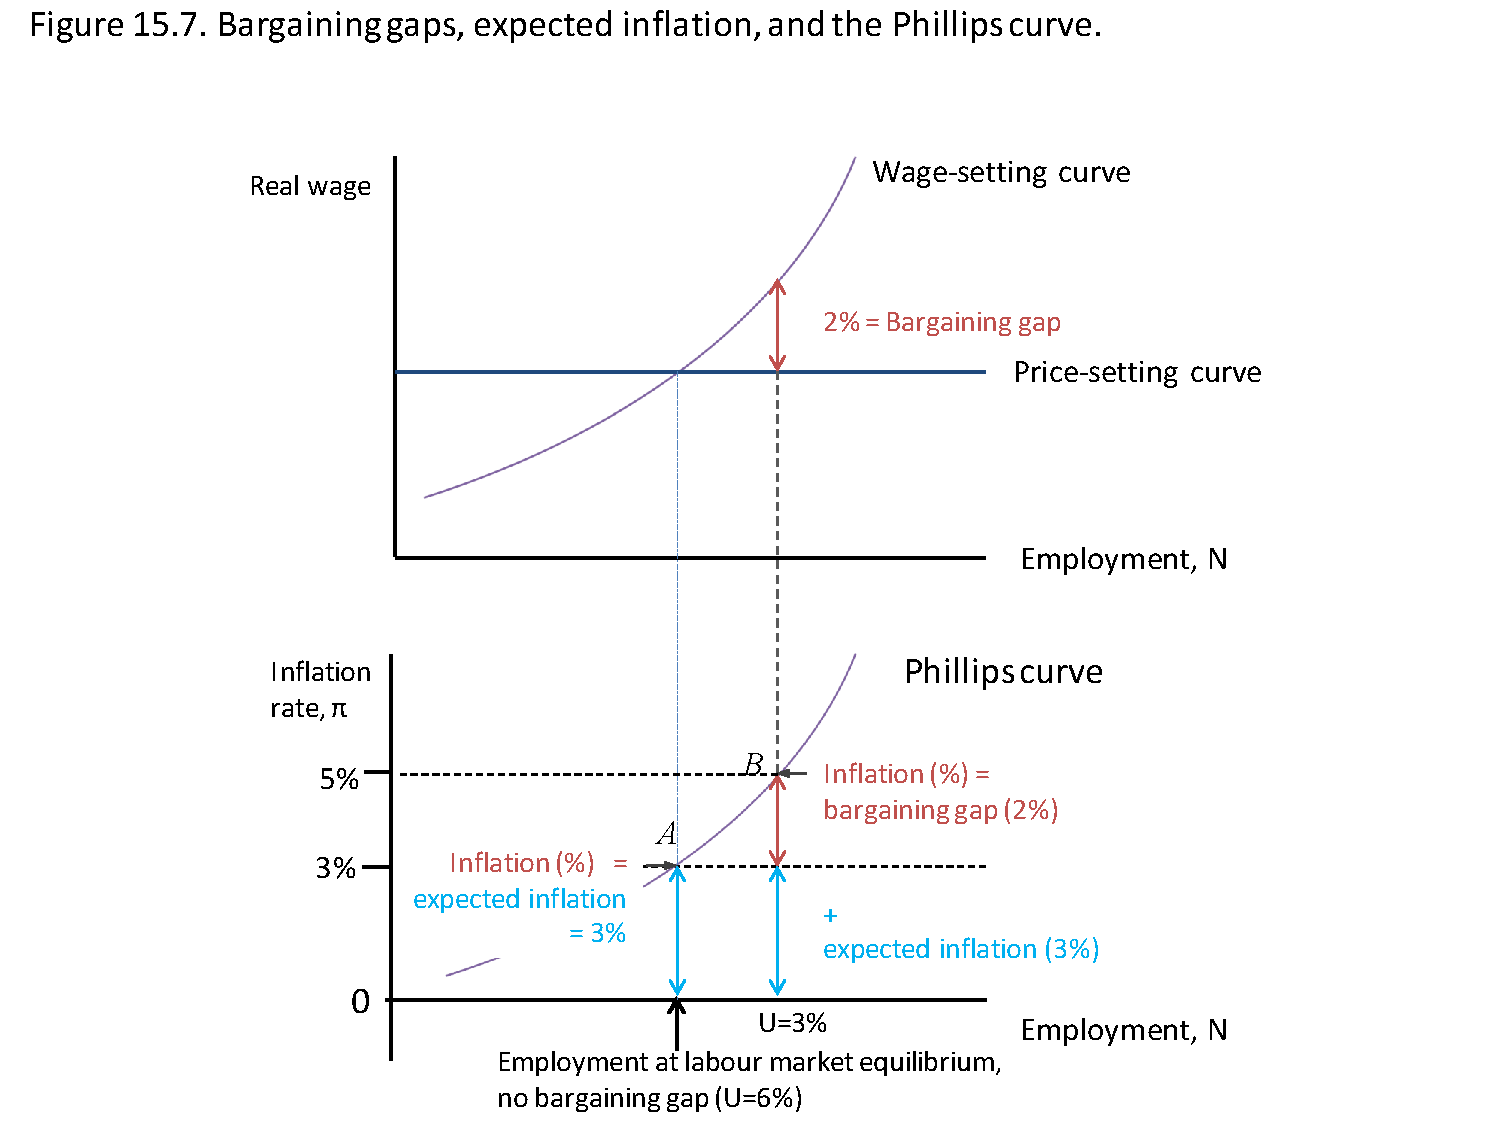
\includegraphics[width=\textwidth]{./figures/10.pdf}
        \end{figure}

    \end{column}
\end{columns}

\end{frame}

\begin{frame}{Expected Inflation Evolves with Positive Bargaining Gap}
\label{slide:Expected_Inflation_Evolves_with_Positive_Bargaining_Gap}
    \begin{figure}
        \centering
        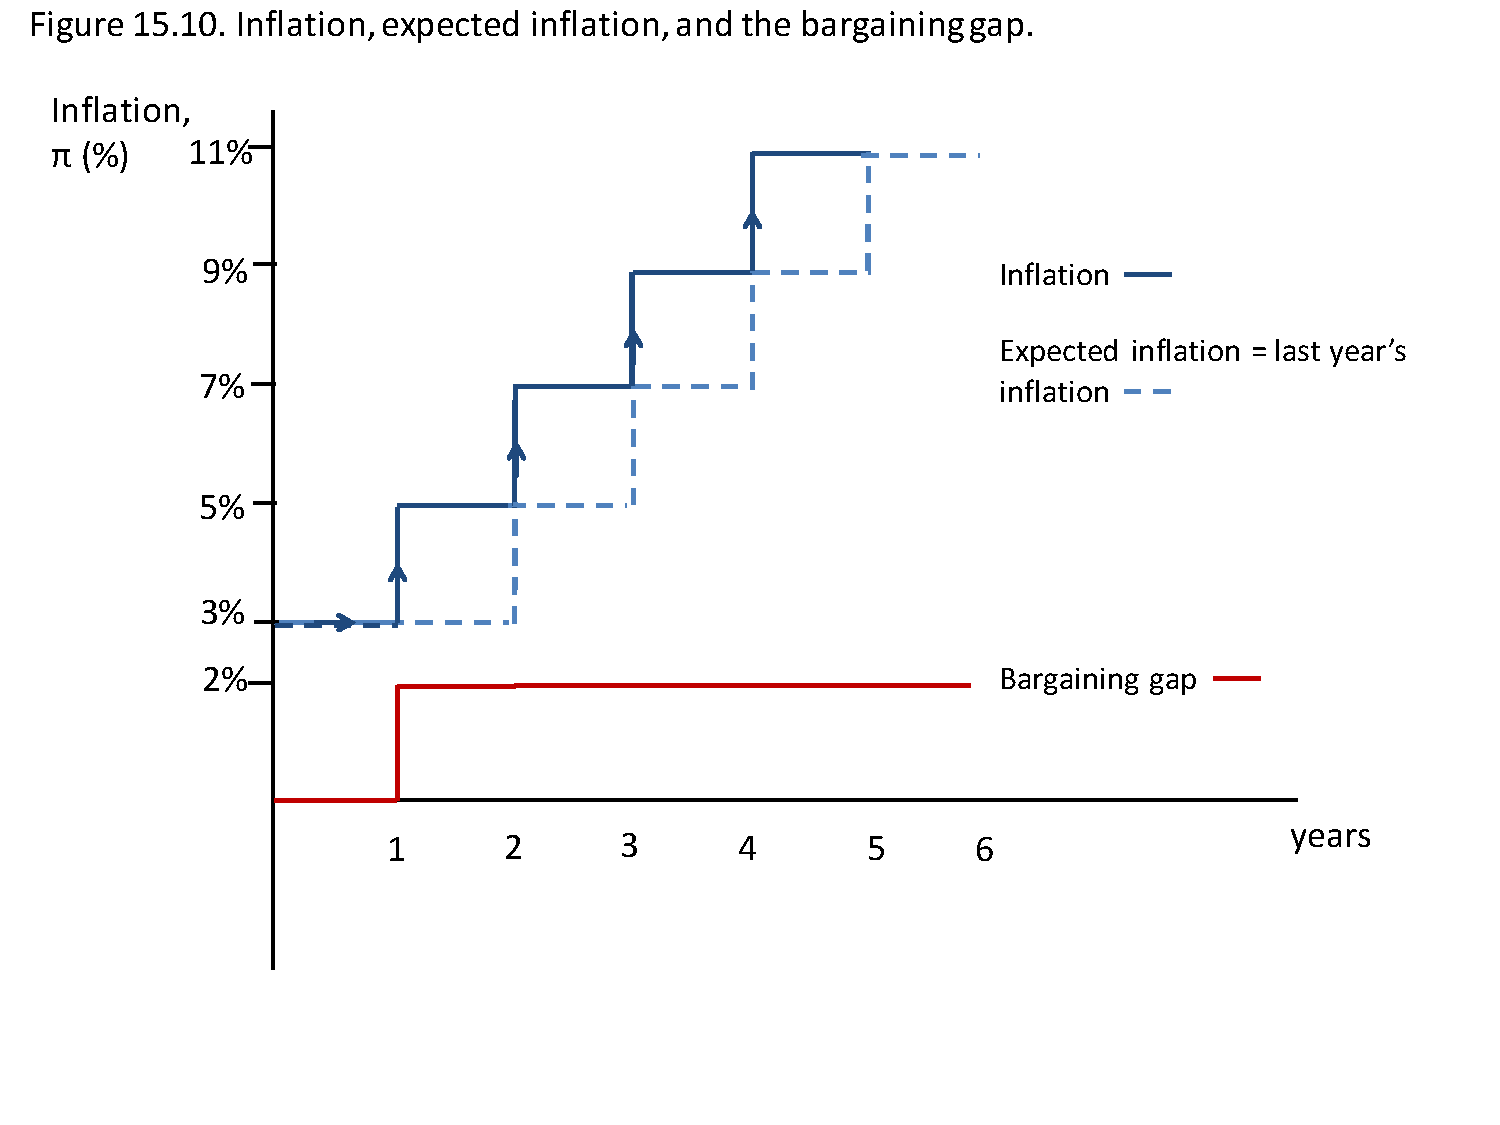
\includegraphics[width=\textwidth]{./figures/13.pdf}
    \end{figure}

\end{frame}

\begin{frame}{Supply Shock}
\label{slide:Supply_Shock}
    \begin{columns}
        \begin{column}{0.4\textwidth}
            \begin{itemize}
                \item Def: unexpected change on the supply-side of the economy
                \begin{itemize}
                    \item e.g. oil price shock.
                \end{itemize}
                \item price of oil $ \uparrow  $
                \item → downward shift of price-setting curve
                \item → prices rise
                \item → real wages fall
                \item → positive bargaining gap
                \item → persistently higher inflation
            \end{itemize}

        \end{column}
        \begin{column}{0.6\textwidth}
            \begin{figure}
                \centering
                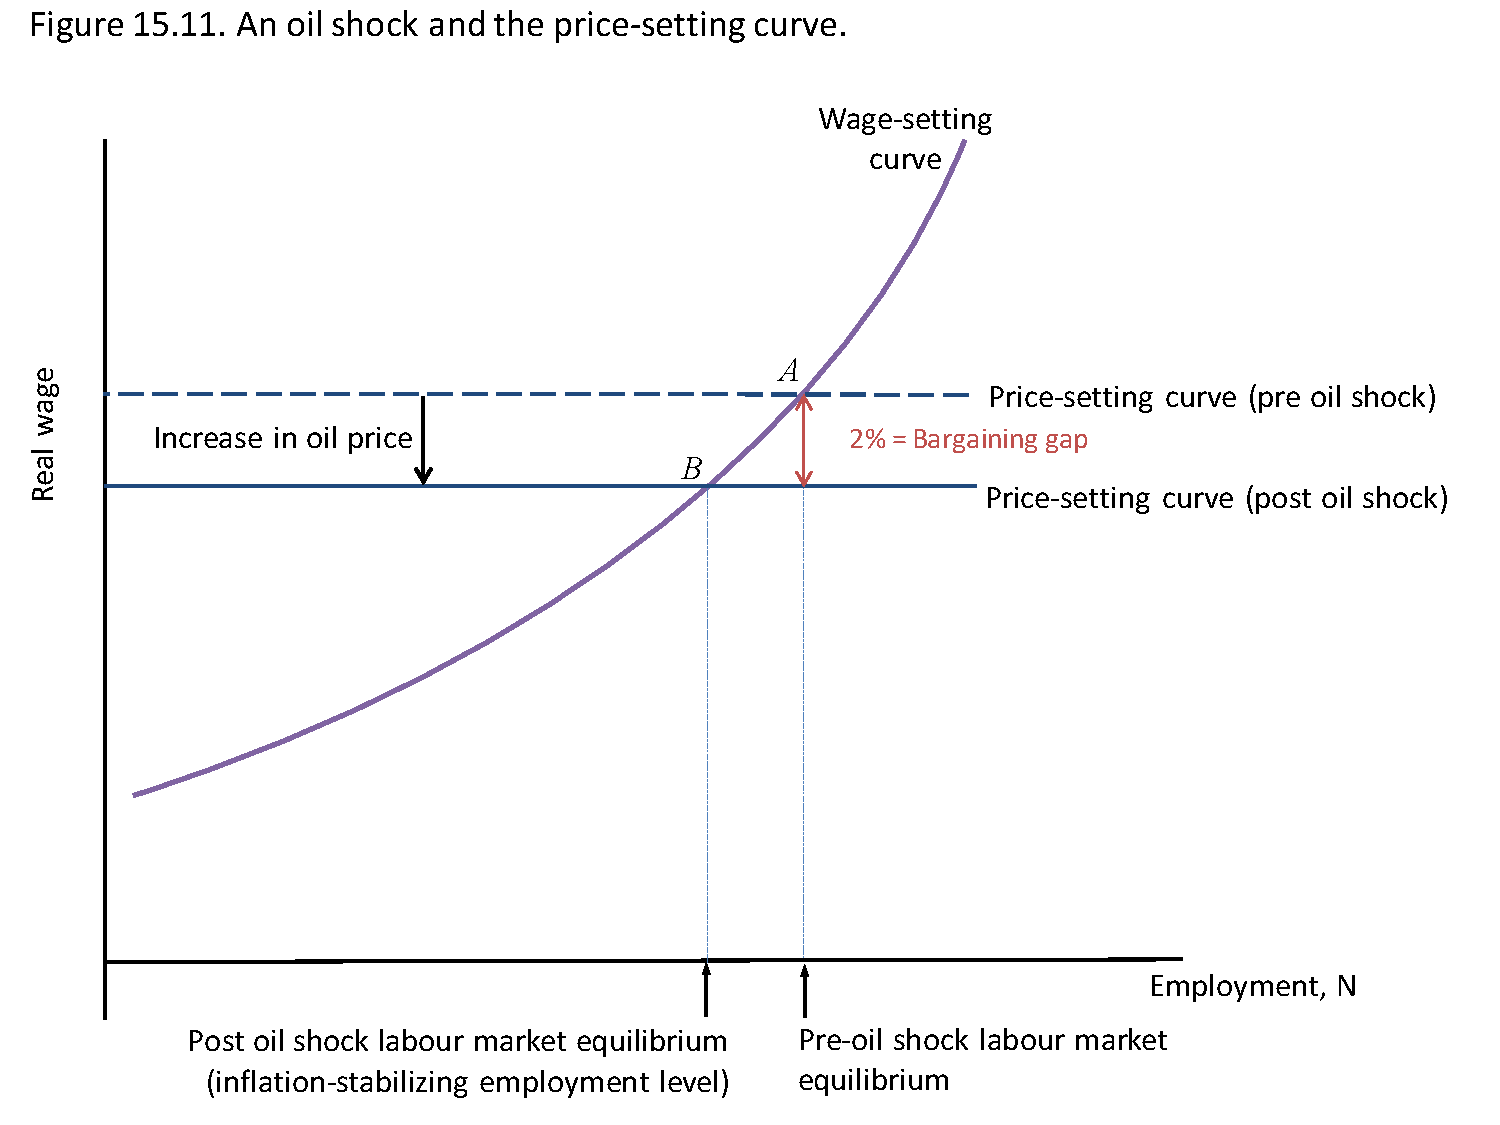
\includegraphics[width=\textwidth]{./figures/14.pdf}
            \end{figure}

        \end{column}
    \end{columns}

\end{frame}

\begin{frame}{Oil Price Shock in 1970s}
\label{slide:Oil_Price_Shock_in_1970s}
    \begin{figure}
        \centering
        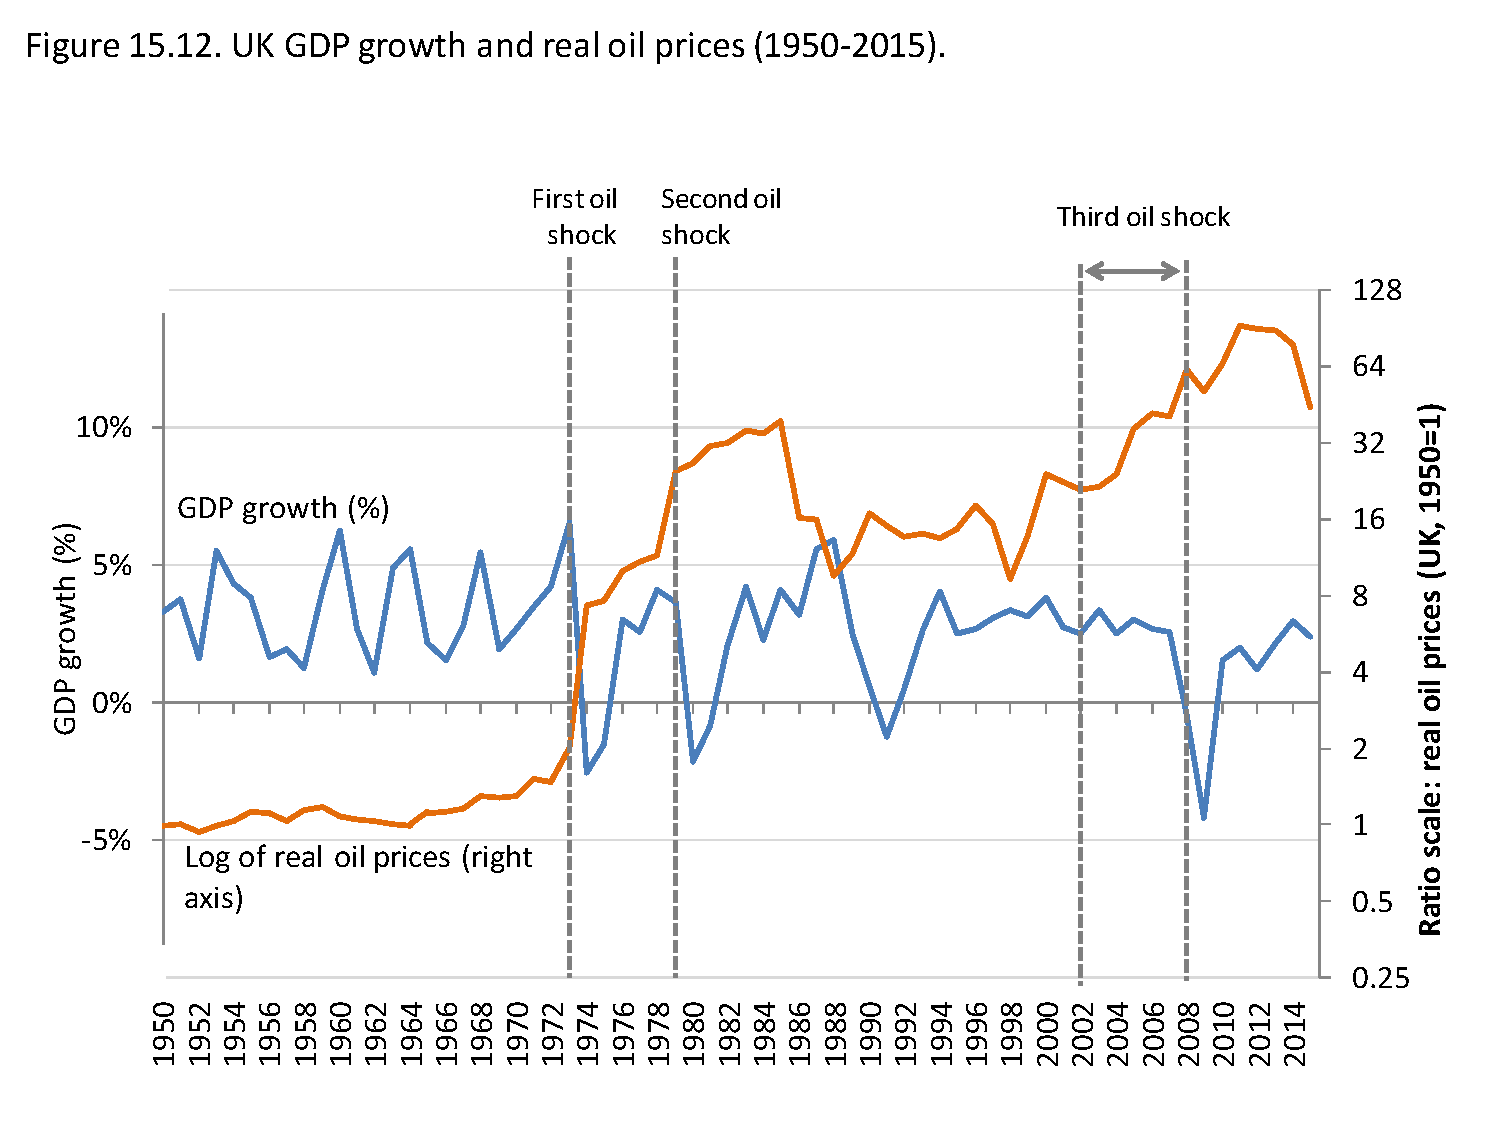
\includegraphics[width=.9\textwidth]{./figures/15.pdf}
    \end{figure}

\end{frame}

\section[Mone]{Monetary Policy}
\label{sec:Monetary_Policy}


\begin{frame}{Transmission Mechanism}
\label{slide:Transmission_Mechanism}
    \begin{figure}
        \centering
        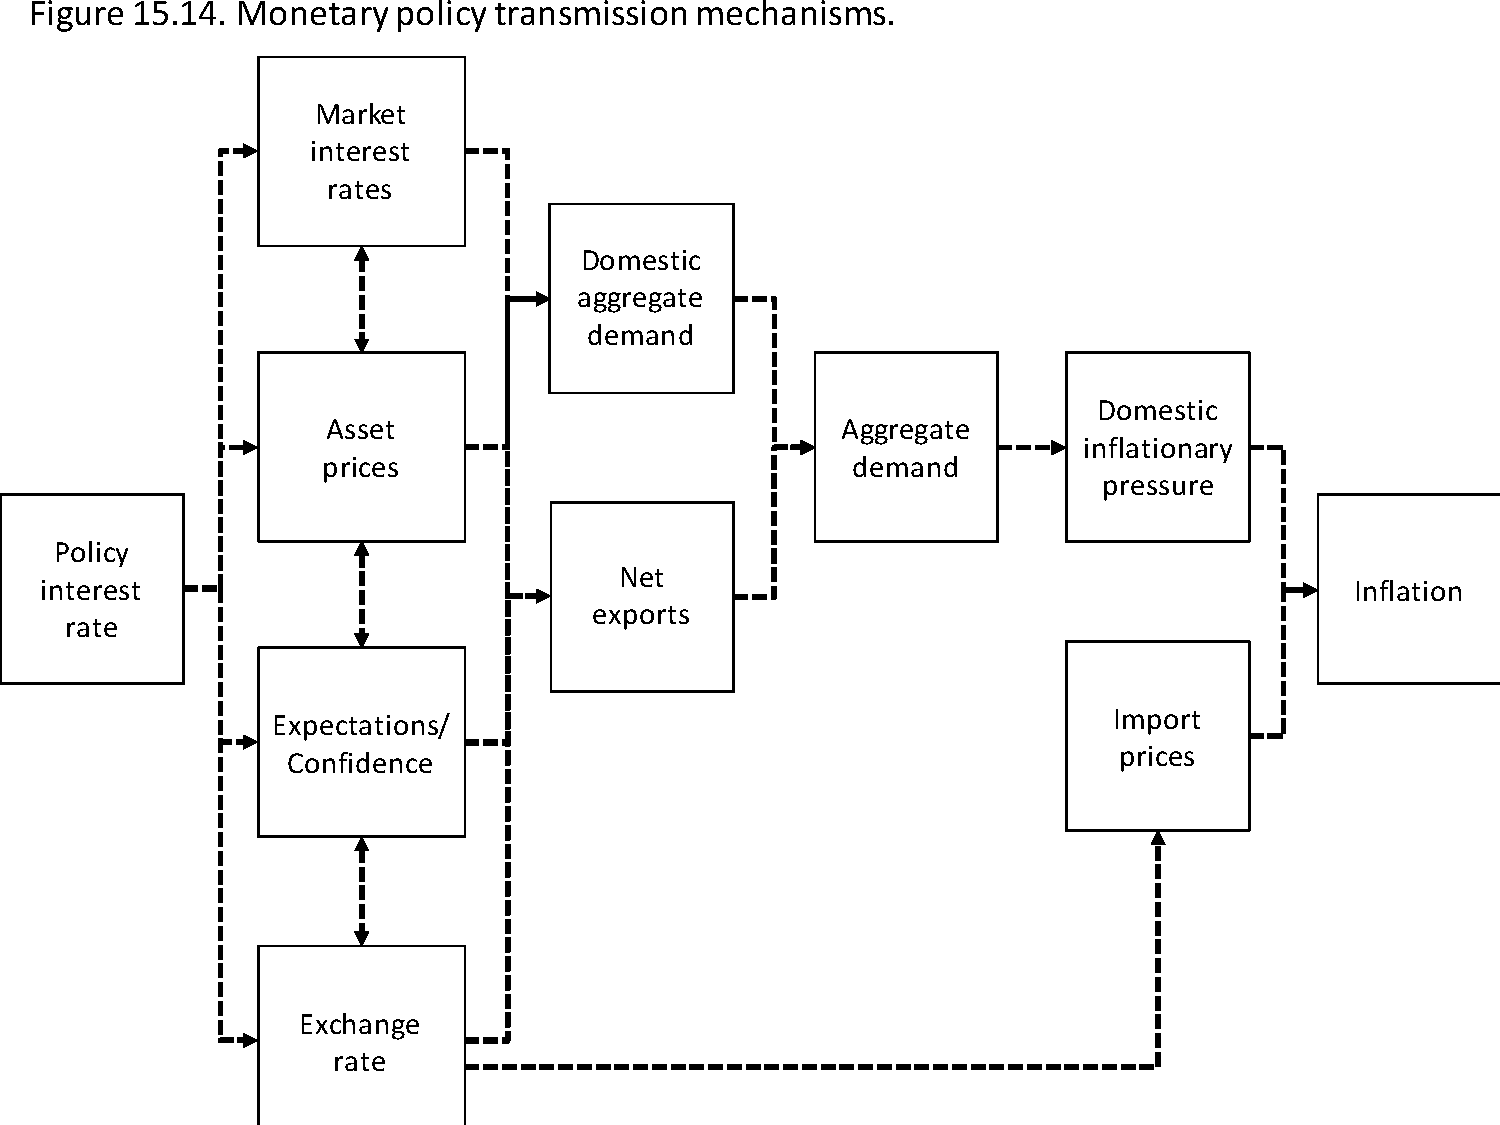
\includegraphics[width=.8\textwidth]{./figures/17.pdf}
    \end{figure}

\end{frame}

\begin{frame}{Market Interest Rates}
\label{slide:Market_Interest_Rates}
    To set the policy rate, the central bank will work backwards:
    \begin{enumerate}
        \item Choose the desired level of aggregate demand, based on the labour market equilibrium and the Phillips curve
        \item Estimate the real interest rate, which will produce this level of aggregate demand (using the multiplier model)
        \item Calculate the nominal policy rate that will produce the appropriate market interest rate.
    \end{enumerate}


\end{frame}

\begin{frame}{Asset prices}
\label{slide:Asset_prices}
    \begin{itemize}
        \item A change in the policy rate has a ripple effect through all the interest rates in the economy.
        \item When the interest rate goes down, the price of assets goes up.
        \item Households who own assets will be wealthier, which will increase their consumption.
    \end{itemize}

\end{frame}

\begin{frame}{Profit expectations}
\label{slide:Profit_expectations}
    \begin{itemize}
        \item Consistent policymaking and good communication with the public builds confidence in the Central Bank.
        \item This can lead firms to expect higher demand and therefore increase investment.
        \item Households may be confident that they will not lose their jobs, and they may increase their consumption.
    \end{itemize}
\end{frame}

\begin{frame}{Exchange rate}
\label{slide:Exchange_rate}
    \begin{itemize}
        \item \textbf{Exchange rate}: number of units of home currency that can be exchanged for one unit of foreign currency.
        \item Interest rates affect demand for home currency in the foreign exchange market, so affects the exchange rate (\textbf{appreciation/depreciation}).
        \item The exchange rate affects relative demand for home-produced goods, so affects net exports.
        \item Therefore, interest rates affect aggregate demand through the market for financial assets.
    \end{itemize}

\end{frame}

\begin{frame}{Exchange rate as transmission mechanism}
\label{slide:Exchange_rate_as_transmission_mechanism}
    \begin{itemize}
        \item Fall in investment ($I$) $ \Rightarrow  $ Fall in AD $ \Rightarrow  $ Fall in forecast inflation
        \item $ \Rightarrow $ Fed cuts interest rate $ \Rightarrow  $ Fall in demand for treasury bill
        \item $ \Rightarrow  $ Fall in demand for USD $ \Rightarrow  $ Depreciation of USD
        \item $ \Rightarrow  $ \green{Exports} (\blue{Imports}) become relatively \green{cheaper} (\blue{expensive})
        \item $ \Rightarrow  $ Increase net export ($ X - M $) $ \Rightarrow  $ increase AD
    \end{itemize}

\end{frame}

\begin{frame}{Monetary policy in the multiplier model}
\label{slide:Monetary_policy_in_the_multiplier_model}
    \begin{figure}
        \centering
        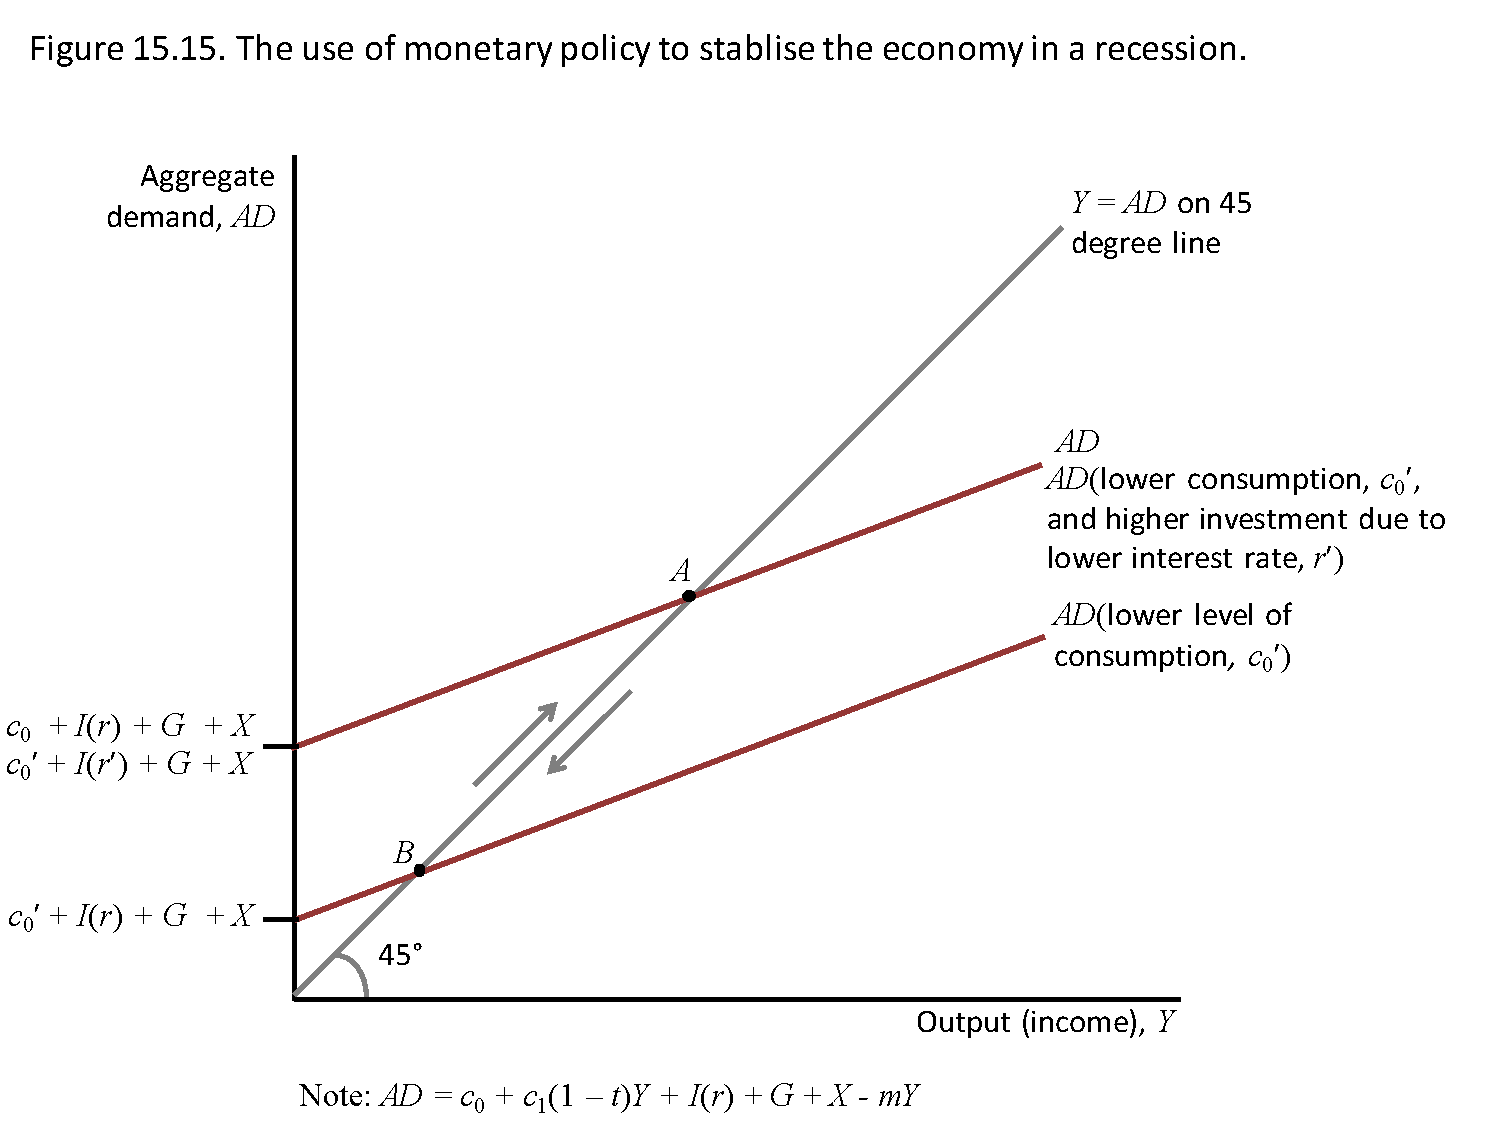
\includegraphics[width=.7\textwidth]{./figures/18.pdf}
    \end{figure}

To stabilize the economy, the central bank stimulates $ I $ by \alert{lowering the real interest rate}. This shifts the aggregate demand curve upward.

\end{frame}

\begin{frame}{Monetary Policy: Limitations}
\label{slide:Monetary_Policy__Limitations}
    \begin{enumerate}
        \item  The short-term nominal interest rate (policy rate) cannot go below zero (``\textbf{zero lower bound}'')
        \begin{itemize}
            \item when the economy is in a slump, a nominal interest rate of zero may not be low enough to stabilize the economy
            \item \textbf{Quantitative easing} = Central bank \alert{purchases} of financial assets aimed at \alert{increasing investment by reducing yields of bond}.
        \end{itemize}
        \item A country without its own currency does not have its own monetary policy
        \begin{itemize}
            \item E.g. countries of the eurozone
        \end{itemize}

    \end{enumerate}


\end{frame}

\begin{frame}{Demand shocks}
\label{slide:Demand_shocks}
    \begin{columns}
        \begin{column}{0.3\textwidth}
            \begin{itemize}
                \item Def: unexpected change in AD
                \item Monetary policy: decreasing the nominal interest rate
                \item Fiscal policy: tax cuts and increased government spending
            \end{itemize}

        \end{column}
        \begin{column}{0.7\textwidth}
            \begin{figure}
                \centering
                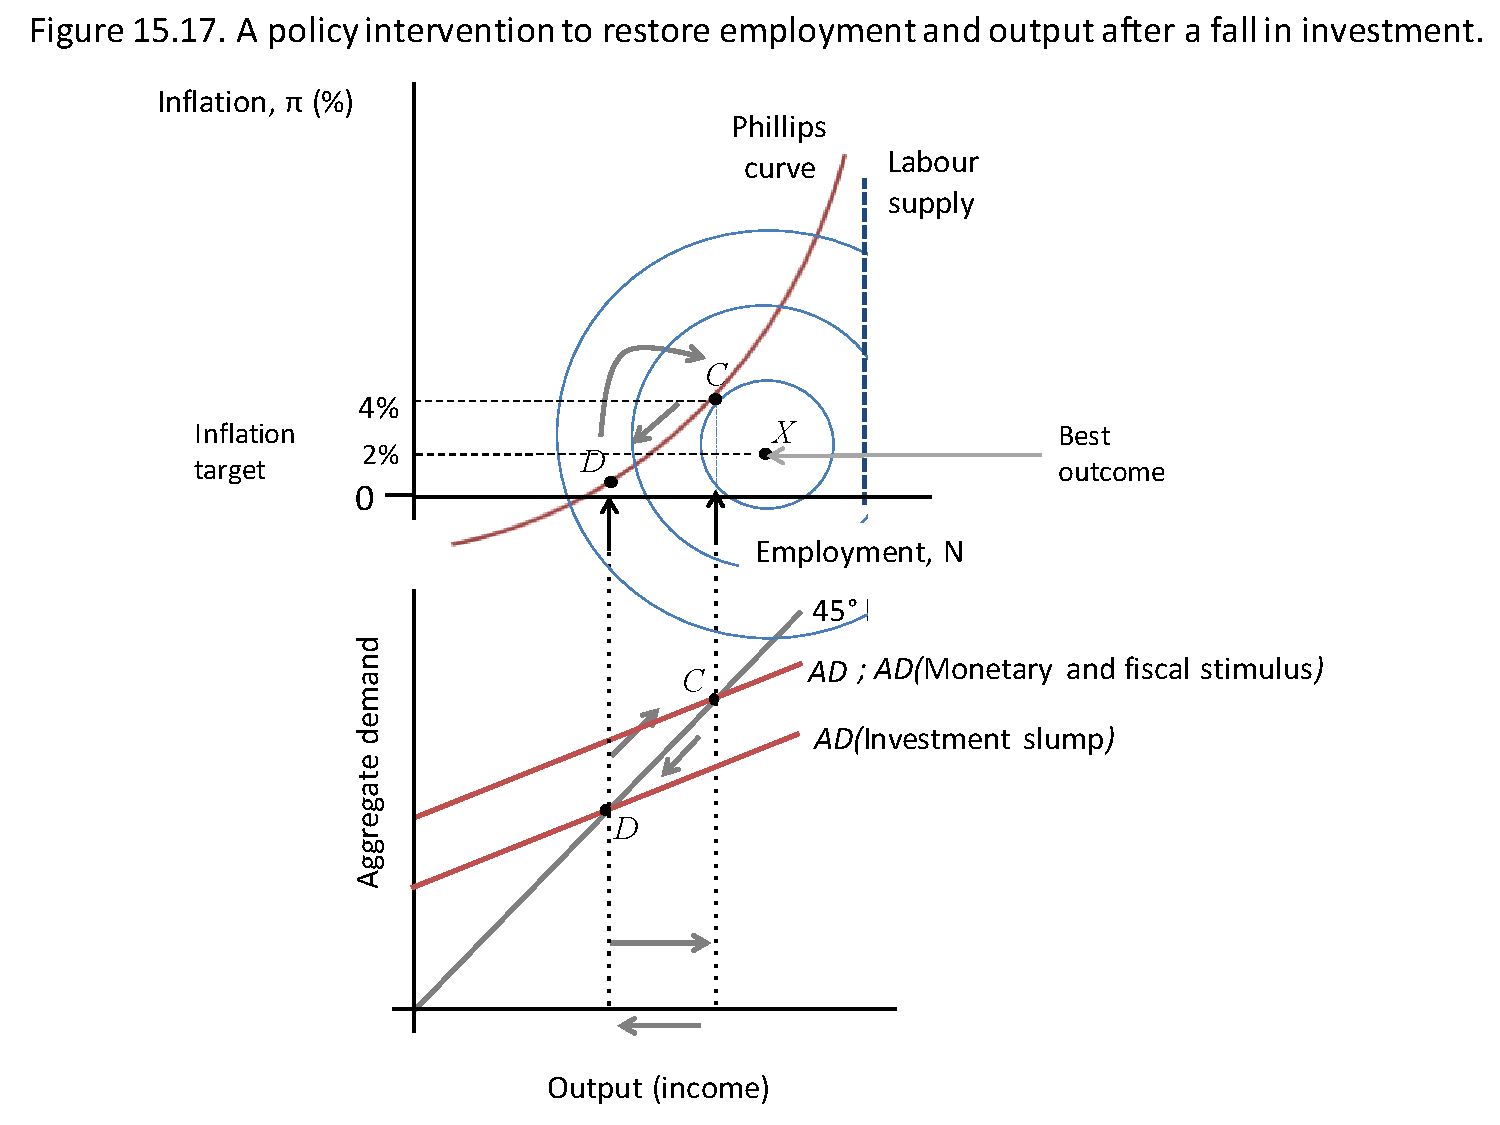
\includegraphics[width=\textwidth]{./figures/20.pdf}
            \end{figure}

        \end{column}
    \end{columns}
\end{frame}


\end{document}
